\chapter{Terahertz (THz) Technology}
\label{ch:thz}

\begin{nontechnical}
\textbf{Think of THz waves as invisible light between microwaves and heat.}

\textbf{Simple idea:}
\begin{itemize}
\item Too fast for traditional electronics ($>$100 GHz)
\item Too slow for optical methods ($<$10 THz)
\item Like X-rays: sees through clothing, plastic, paper
\item Unlike X-rays: completely safe (no ionizing radiation)
\end{itemize}

\textbf{Real use:} Airport body scanners use THz to detect hidden objects without harmful radiation. Your security screening likely uses this technology.

\textbf{The catch:} Water blocks THz completely. That's why it can't penetrate deep into your body (we're 70\% water) and why it doesn't work well in rain or fog. This is actually a safety feature!
\end{nontechnical}

\section{Overview}

\textbf{Terahertz (THz) technology} operates in the electromagnetic spectrum between 0.1 and 10~THz (100~GHz to 10,000~GHz), bridging the gap between microwave electronics and optical photonics.

\begin{keyconcept}
The \textbf{``THz gap''} represents a historically challenging frequency range where neither pure electronic nor pure optical techniques work efficiently. Modern quantum cascade lasers and photoconductive methods have revolutionized this field, enabling practical THz systems for imaging, spectroscopy, and communications.
\end{keyconcept}

THz radiation exhibits unique properties: transparency through many materials (plastics, clothing, paper), strong absorption by water and metals, and non-ionizing photon energies that make it safe for biological applications.

\section{Mathematical Description}

\subsection{Frequency Range and Photon Energy}

The THz region spans the electromagnetic spectrum between microwave and infrared:
\begin{equation}
f_{\text{THz}} = 0.1 \text{ to } 10 \text{ THz} = 10^{11} \text{ to } 10^{13} \text{ Hz}
\end{equation}
where:
\begin{itemize}
\item $f_{\text{THz}}$ = terahertz frequency (Hz)
\item Lower bound: 100~GHz (overlaps with millimeter wave)
\item Upper bound: 10~THz (transitions to far-infrared)
\end{itemize}

\textbf{Corresponding wavelength range:}
\begin{equation}
\lambda = \frac{c}{f} = \frac{3 \times 10^8 \text{ m/s}}{f_{\text{THz}}}
\end{equation}
yielding:
\begin{itemize}
\item At 0.1~THz: $\lambda = 3$~mm
\item At 1~THz: $\lambda = 300$~$\mu$m
\item At 10~THz: $\lambda = 30$~$\mu$m
\end{itemize}

\textbf{Photon energy:}
\begin{equation}
E_{\text{photon}} = hf
\end{equation}
where:
\begin{itemize}
\item $h = 6.626 \times 10^{-34}$~J$\cdot$s (Planck's constant)
\item $f$ = frequency (Hz)
\end{itemize}

At 1~THz, the photon energy is:
\begin{equation}
E = (6.626 \times 10^{-34})(10^{12}) = 6.626 \times 10^{-22} \text{ J} = 4.1 \text{ meV}
\end{equation}

\begin{calloutbox}{Why THz is Non-Ionizing}
With photon energies in the meV range, THz radiation is \textbf{far below} the $\sim$eV threshold needed to ionize atoms or break chemical bonds. This makes THz inherently safe for biological applications, unlike UV or X-rays which operate at keV energies.
\end{calloutbox}

\subsection{The THz Gap}

Historically, the THz region was difficult to access:
\begin{equation}
\text{THz Gap} = \begin{cases}
f < 100 \text{ GHz} & \text{Electronic devices dominant} \\
0.1 < f < 10 \text{ THz} & \text{Hybrid approaches needed} \\
f > 10 \text{ THz} & \text{Optical techniques dominant}
\end{cases}
\end{equation}

This gap exists because:
\begin{itemize}
\item \textbf{Electronics:} Transistor cutoff frequencies $f_T < 1$~THz typically
\item \textbf{Optics:} Laser transitions too high energy for THz ($>$100~THz)
\item \textbf{Solution:} Quantum cascade lasers (QCLs) bridge the gap
\end{itemize}

\section{THz Generation and Detection}

\subsection{THz Spectrum Overview}

The THz region bridges electronics and photonics:

\begin{center}
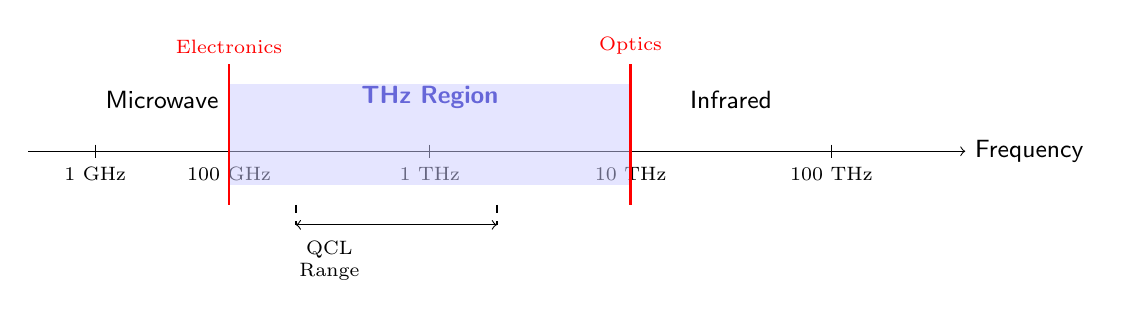
\begin{tikzpicture}[scale=0.85]
% Frequency axis
\draw[->] (0,0) -- (14,0) node[right] {\sffamily\small Frequency};

% Frequency markers
\foreach \x/\label in {1/1 GHz, 3/100 GHz, 6/1 THz, 9/10 THz, 12/100 THz} {
    \draw (\x,0.1) -- (\x,-0.1) node[below,font=\scriptsize] {\label};
}

% Region labels
\node[above,font=\sffamily\small] at (2,0.5) {Microwave};
\node[above,font=\sffamily\small,blue!70!black] at (6,0.5) {\textbf{THz Region}};
\node[above,font=\sffamily\small] at (10.5,0.5) {Infrared};

% Shaded THz region
\fill[blue!20,opacity=0.5] (3,-0.5) rectangle (9,1);

% Technology boundaries
\draw[thick,red] (3,-0.8) -- (3,1.3) node[above,font=\scriptsize,text=red] {Electronics};
\draw[thick,red] (9,-0.8) -- (9,1.3) node[above,font=\scriptsize,text=red] {Optics};

% Applications
\node[below,font=\scriptsize,align=center] at (4.5,-1.2) {QCL\\Range};
\draw[thick,dashed] (4,-0.8) -- (4,-1.1);
\draw[thick,dashed] (7,-0.8) -- (7,-1.1);
\draw[<->] (4,-1.1) -- (7,-1.1);
\end{tikzpicture}
\end{center}

\subsection{Quantum Cascade Lasers (QCLs)}

\textbf{Principle:} QCLs use engineered quantum wells to generate THz radiation through intersubband transitions.

\subsubsection{QCL Structure}

\begin{center}
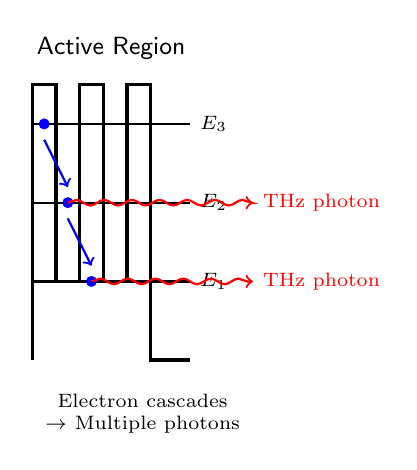
\begin{tikzpicture}[scale=1.0]
% Energy levels
\draw[thick] (0,3) -- (2,3) node[right] {\scriptsize $E_3$};
\draw[thick] (0,2) -- (2,2) node[right] {\scriptsize $E_2$};
\draw[thick] (0,1) -- (2,1) node[right] {\scriptsize $E_1$};

% Quantum well barriers
\draw[very thick] (0,0) -- (0,3.5) -- (0.3,3.5) -- (0.3,1) -- (0.6,1) -- (0.6,3.5) -- (0.9,3.5) -- (0.9,1) -- (1.2,1) -- (1.2,3.5) -- (1.5,3.5) -- (1.5,0) -- (2,0);

% Electron
\fill[blue] (0.15,3) circle (2pt);
\fill[blue] (0.45,2) circle (2pt);
\fill[blue] (0.75,1) circle (2pt);

% THz photon emissions
\draw[->,thick,red,decorate,decoration={snake,amplitude=1pt}] (0.45,2) -- (2.8,2) node[right,font=\scriptsize] {THz photon};
\draw[->,thick,red,decorate,decoration={snake,amplitude=1pt}] (0.75,1) -- (2.8,1) node[right,font=\scriptsize] {THz photon};

% Arrows showing cascade
\draw[->,thick,blue] (0.15,2.8) -- (0.45,2.2);
\draw[->,thick,blue] (0.45,1.8) -- (0.75,1.2);

% Labels
\node[above,font=\sffamily\small] at (1,3.7) {Active Region};
\node[below,font=\scriptsize,align=center] at (1.4,-0.3) {Electron cascades\\$\rightarrow$ Multiple photons};
\end{tikzpicture}
\end{center}

\textbf{Energy level design:}
\begin{equation}
\Delta E = E_3 - E_2 = hf_{\text{THz}}
\end{equation}
where:
\begin{itemize}
\item $\Delta E$ = intersubband energy spacing (meV)
\item $E_3, E_2$ = engineered quantum well energy levels
\item $f_{\text{THz}}$ = desired THz emission frequency
\end{itemize}

\textbf{Output power:}
\begin{equation}
P_{\text{out}} = \eta \cdot I \cdot V \cdot N_{\text{stages}}
\end{equation}
where:
\begin{itemize}
\item $\eta$ = wall-plug efficiency (0.5--5\%)
\item $I$ = drive current (typically 100--1000~mA)
\item $V$ = voltage per stage ($\sim$10--20~mV)
\item $N_{\text{stages}}$ = number of cascaded stages (100--300)
\end{itemize}

\begin{warningbox}
Most THz QCLs require \textbf{cryogenic cooling} (77~K or below) for efficient operation. Room-temperature THz QCLs exist but have significantly reduced power output ($<$1~mW) and limited frequency range.
\end{warningbox}

\subsection{THz System Block Diagram}

A complete THz imaging system:

\begin{center}
\begin{tikzpicture}[
  block/.style={rectangle, draw, minimum width=2cm, minimum height=0.9cm, font=\sffamily\small},
  node distance=2cm,
  font=\small
]
% Transmitter chain
\node[block] (qcl) {QCL\\Source};
\node[block, right of=qcl] (modulator) {Amplitude\\Modulator};
\node[block, right of=modulator] (txant) {TX\\Antenna};

% Free space
\node[right of=txant, node distance=2.2cm] (space) {\sffamily Target};

% Receiver chain
\node[block, right of=space, node distance=2.2cm] (rxant) {RX\\Antenna};
\node[block, right of=rxant] (mixer) {Detector\\(Bolometer)};
\node[block, right of=mixer] (proc) {Signal\\Processing};

% Arrows
\draw[->,thick] (qcl) -- node[above,font=\tiny] {CW THz} (modulator);
\draw[->,thick] (modulator) -- node[above,font=\tiny] {modulated} (txant);
\draw[->,thick,red,decorate,decoration={snake,amplitude=1pt}] (txant) -- (space);
\draw[->,thick,red,decorate,decoration={snake,amplitude=1pt}] (space) -- node[above,font=\tiny] {reflected} (rxant);
\draw[->,thick] (rxant) -- (mixer);
\draw[->,thick] (mixer) -- node[above,font=\tiny] {baseband} (proc);

% Control signal
\node[block, below=1.4cm of modulator] (drive) {Drive\\Electronics};
\draw[->,thick] (drive) -- (modulator);
\draw[->,thick] (drive) -- (qcl);

% Lock-in reference
\draw[->,thick,dashed] (drive.east) -| (proc.south) node[pos=0.25,right,font=\tiny] {ref};

% Labels
\node[above,font=\sffamily\small] at (modulator.north) [yshift=0.7cm] {Transmitter};
\node[above,font=\sffamily\small] at (mixer.north) [yshift=0.7cm] {Receiver};
\end{tikzpicture}
\end{center}

\subsection{Other THz Sources}

\subsubsection{Photoconductive Antennas}

Generate pulsed THz via femtosecond laser excitation:
\begin{equation}
P_{\text{THz}}(t) \propto \frac{\partial J(t)}{\partial t}
\end{equation}
where $J(t)$ is the photogenerated current transient.

\textbf{Characteristics:}
\begin{itemize}
\item Broadband output: 0.1--5~THz
\item Low average power: $\sim$$\mu$W range
\item Enables time-domain spectroscopy (THz-TDS)
\end{itemize}

\subsubsection{Frequency Multiplication}

Electronic approach using nonlinear devices:
\begin{equation}
f_{\text{out}} = N \times f_{\text{in}}
\end{equation}
where:
\begin{itemize}
\item $N$ = multiplication factor (typically 2--9)
\item $f_{\text{in}}$ = input microwave frequency (10--100~GHz)
\item Efficiency: $\eta \propto N^{-2}$ (drops rapidly with $N$)
\end{itemize}

\textbf{Advantage:} Room temperature, compact\\
\textbf{Limitation:} Practical only below $\sim$1~THz

\subsection{THz Detection Methods}

\subsubsection{Direct Detection}

Thermal detectors (bolometers):
\begin{equation}
\Delta R = \alpha \cdot P_{\text{THz}} \cdot R_{\text{bias}}
\end{equation}
where:
\begin{itemize}
\item $\Delta R$ = resistance change
\item $\alpha$ = temperature coefficient of resistance
\item $P_{\text{THz}}$ = incident THz power
\end{itemize}

\textbf{Typical NEP:} $10^{-12}$ to $10^{-14}$~W/Hz$^{1/2}$

\subsubsection{Coherent Detection}

Heterodyne detection for spectral information:
\begin{equation}
f_{\text{IF}} = |f_{\text{THz}} - f_{\text{LO}}|
\end{equation}
where:
\begin{itemize}
\item $f_{\text{IF}}$ = intermediate frequency (MHz--GHz)
\item $f_{\text{LO}}$ = local oscillator frequency
\item Provides phase and amplitude information
\end{itemize}

\section{Propagation Characteristics}

\subsection{Atmospheric Attenuation}

THz propagation is dominated by water vapor absorption:
\begin{equation}
\alpha(f) = \alpha_{\text{dry}}(f) + \rho \cdot \alpha_{\text{H}_2\text{O}}(f)
\end{equation}
where:
\begin{itemize}
\item $\alpha(f)$ = total attenuation coefficient (dB/km)
\item $\alpha_{\text{dry}}(f)$ = dry air contribution
\item $\rho$ = water vapor density (g/m$^3$)
\item $\alpha_{\text{H}_2\text{O}}(f)$ = water vapor absorption cross-section
\end{itemize}

\textbf{Typical attenuation values:}

\begin{center}
\begin{tabular}{@{}lll@{}}
\toprule
Frequency & Attenuation & Usability \\
\midrule
0.3~THz & 10--20~dB/km & Good (communications) \\
1.0~THz & 100--200~dB/km & Limited range \\
2.0~THz & $>$500~dB/km & Indoor only \\
\bottomrule
\end{tabular}
\end{center}

\textbf{Transmission windows:} 0.35, 0.85, 1.4~THz (local minima in absorption)

\subsection{Link Budget}

Total path loss for THz link:
\begin{equation}
L_{\text{total}} = L_{\text{FSPL}} + L_{\text{atm}} + L_{\text{misc}}
\end{equation}

\textbf{Free-space path loss:}
\begin{equation}
L_{\text{FSPL}} = 20\log_{10}(d) + 20\log_{10}(f) + 20\log_{10}\left(\frac{4\pi}{c}\right)
\end{equation}
where:
\begin{itemize}
\item $d$ = distance (m)
\item $f$ = frequency (Hz)
\item $c = 3 \times 10^8$~m/s
\end{itemize}

\textbf{Example at 1~THz, 1~km:}
\begin{equation}
L_{\text{FSPL}} = 20\log_{10}(1000) + 20\log_{10}(10^{12}) + 32.45 = 152 \text{ dB}
\end{equation}

\textbf{Atmospheric contribution:}
\begin{equation}
L_{\text{atm}} = \alpha(f) \cdot d = 150 \text{ dB/km} \times 1 \text{ km} = 150 \text{ dB}
\end{equation}

\textbf{Total loss:} $\sim$300~dB (extreme!)

\begin{calloutbox}{THz Communication Range}
The extreme path loss ($>$250~dB at 1~THz over 1~km) limits THz communications to:
\begin{itemize}
\item Indoor environments ($<$100~m)
\item Vacuum/space applications (no atmospheric loss)
\item Very high transmit power systems (FEL-based)
\end{itemize}
\end{calloutbox}

\subsection{Material Penetration}

Skin depth in materials:
\begin{equation}
\delta = \frac{1}{\alpha} = \frac{1}{\frac{4\pi f}{c}\sqrt{\epsilon_r \tan\delta}}
\end{equation}
where:
\begin{itemize}
\item $\delta$ = penetration depth (m)
\item $\epsilon_r$ = relative permittivity
\item $\tan\delta$ = loss tangent
\end{itemize}

\textbf{Typical penetration depths at 1~THz:}

\begin{center}
\begin{tabular}{@{}ll@{}}
\toprule
Material & Penetration Depth \\
\midrule
Plastics (PE, PTFE) & cm to m \\
Dry paper & $\sim$1~cm \\
Clothing (cotton) & $\sim$1~cm \\
\textbf{Water} & \textbf{$\sim$100~$\mu$m} \\
Metals & $\sim$1~nm (reflective) \\
\bottomrule
\end{tabular}
\end{center}

\begin{keyconcept}
\textbf{Water is the THz blocker.} With $\delta \approx 100$~$\mu$m, THz cannot penetrate:
\begin{itemize}
\item Deep into biological tissue (70\% water)
\item Through rain or fog
\item Across humid outdoor environments
\end{itemize}
This property enables safe imaging (surface only) but limits range.
\end{keyconcept}

\section{Biological Interactions and Safety}

\subsection{Tissue Penetration}

Human tissue has high water content ($\sim$70\%), leading to strong absorption:
\begin{equation}
\delta_{\text{tissue}} = \frac{c}{4\pi f \sqrt{\epsilon_r \epsilon''_r}}
\end{equation}
where:
\begin{itemize}
\item $\delta_{\text{tissue}}$ = penetration depth in tissue (m)
\item $\epsilon''_r$ = imaginary permittivity (loss factor)
\item For water-rich tissue: $\epsilon''_r \approx 10$--20 at 1~THz
\end{itemize}

\textbf{Penetration depths at 1~THz:}

\begin{center}
\begin{tabular}{@{}ll@{}}
\toprule
Tissue Type & Penetration Depth \\
\midrule
Skin (epidermis) & 0.5--1~mm \\
Fat (adipose) & $\sim$2~mm \\
Muscle & 0.3--0.5~mm \\
Bone & $\sim$1~mm \\
Brain tissue & $\sim$0.5~mm \\
\bottomrule
\end{tabular}
\end{center}

\subsection{Safety and Bioeffects}

\subsubsection{Primary Effect: Thermal Heating}

Power deposition in tissue:
\begin{equation}
\frac{dT}{dt} = \frac{\alpha \cdot I}{c_p \cdot \rho}
\end{equation}
where:
\begin{itemize}
\item $T$ = temperature (K)
\item $\alpha$ = absorption coefficient (m$^{-1}$)
\item $I$ = THz intensity (W/m$^2$)
\item $c_p$ = specific heat capacity (J/kg$\cdot$K)
\item $\rho$ = tissue density (kg/m$^3$)
\end{itemize}

\textbf{Typical heating:} $\sim$0.1--1~°C at safety-compliant exposures

\subsubsection{Safety Standards}

IEEE/ICNIRP exposure limits for continuous wave THz:
\begin{equation}
S_{\text{max}} = \begin{cases}
10 \text{ mW/cm}^2 & 0.3 \text{ THz} \\
10 \text{ mW/cm}^2 & 1 \text{ THz} \\
100 \text{ mW/cm}^2 & 3 \text{ THz (IR transition)}
\end{cases}
\end{equation}
where $S_{\text{max}}$ is the maximum power density for 6-minute averaged exposure.

\textbf{Rationale:}
\begin{itemize}
\item Surface absorption prevents deep tissue damage
\item Thermal effects are well-understood and controllable
\item No evidence of non-thermal bioeffects at safe power levels
\end{itemize}

\begin{warningbox}
While THz is non-ionizing and generally safe, \textbf{eye safety} is critical:
\begin{itemize}
\item Cornea is transparent to THz (low water content)
\item Direct exposure can damage lens proteins
\item Always use beam blocks and safety interlocks
\end{itemize}
\end{warningbox}

\subsection{Speculative Non-Thermal Effects}

Current research investigates potential resonant effects:
\begin{equation}
f_{\text{resonance}} = \frac{1}{2\pi\sqrt{LC_{\text{molecular}}}}
\end{equation}

\textbf{Hypotheses (not proven):}
\begin{itemize}
\item Resonant excitation of protein vibrational modes
\item Perturbation of hydrogen bond networks
\item Effects on DNA conformational dynamics
\end{itemize}

\textbf{Consensus:} At safety-compliant power levels, thermal effects dominate.

\section{Applications}

\subsection{Security Screening}

\textbf{Airport body scanners} use THz imaging for concealed object detection.

\textbf{System parameters:}
\begin{itemize}
\item Frequency: 0.2--0.4~THz (L-band THz)
\item Power: $<$1~mW (eye-safe)
\item Scan time: 2--3 seconds (full body)
\item Resolution: $\sim$5~mm
\end{itemize}

\textbf{Advantages over X-rays:}
\begin{itemize}
\item Non-ionizing (no DNA damage risk)
\item Surface penetration only (privacy-preserving)
\item Detects non-metallic threats (explosives, ceramics)
\end{itemize}

\textbf{Deployed systems:}
\begin{itemize}
\item Smiths Detection eqo scanner
\item Rohde \& Schwarz QPS systems
\item Used in $>$1000 airports worldwide
\end{itemize}

\subsection{THz Spectroscopy}

Molecular identification via rotational/vibrational resonances:
\begin{equation}
\alpha(f) = \sum_i S_i \cdot g(f - f_i)
\end{equation}
where:
\begin{itemize}
\item $S_i$ = line strength for transition $i$
\item $f_i$ = molecular resonance frequency
\item $g(f)$ = line shape function (Lorentzian/Gaussian)
\end{itemize}

\textbf{Applications:}
\begin{itemize}
\item \textbf{Pharmaceutical QC:} Identify polymorphs, detect counterfeits
\item \textbf{Explosives detection:} TNT, RDX have unique THz signatures
\item \textbf{Gas sensing:} ppb-level sensitivity for H$_2$O, CO, NO$_x$
\end{itemize}

\begin{calloutbox}{Real-World Example: Pfizer Quality Control}
Pfizer uses THz spectroscopy to non-destructively verify tablet composition through packaging. Detection accuracy: $>$99\% for active pharmaceutical ingredients (APIs).
\end{calloutbox}

\subsection{Medical Imaging}

\textbf{Skin cancer detection:}
\begin{itemize}
\item Frequency: 0.5--1~THz
\item Contrast mechanism: Water content difference (tumor vs normal)
\item Resolution: $\sim$0.3~mm (better than MRI)
\item Penetration: 1--2~mm (early-stage detection)
\end{itemize}

\textbf{Burn assessment:}
\begin{itemize}
\item Differentiates burn depth (1st, 2nd, 3rd degree)
\item Non-contact imaging (avoids pain)
\item Real-time feedback for surgeons
\end{itemize}

\subsection{THz Communications}

Wireless data rates approaching 1~Tbps:
\begin{equation}
C = B \cdot \log_2(1 + \text{SNR})
\end{equation}

\textbf{6G vision:}
\begin{itemize}
\item Frequency bands: 0.1--0.3~THz (allocated)
\item Indoor range: 10--100~m
\item Target data rate: 100~Gbps to 1~Tbps
\item Modulation: 64-QAM, OFDM
\end{itemize}

\textbf{Challenges:}
\begin{itemize}
\item Atmospheric loss ($>$100~dB/km)
\item Phase noise (LO stability critical)
\item Device technology (PA power limited)
\end{itemize}

\subsection{Art Conservation}

THz imaging reveals hidden layers in paintings:
\begin{itemize}
\item Non-invasive (no sampling)
\item Penetrates paint layers (1--2~mm)
\item Detects underdrawings, pentimenti, restorations
\end{itemize}

\textbf{Example:} Van Gogh's "Patch of Grass" revealed hidden portrait using THz imaging (2008).

\section{Worked Example: THz Imaging System Link Budget}

\textbf{Scenario:} Design a THz imaging system for security screening at 0.3~THz

\subsection*{Given Parameters}

\begin{tabular}{@{}ll@{}}
Frequency & $f = 0.3$~THz = 300~GHz \\
TX power & $P_t = 1$~mW = 0~dBm \\
TX antenna gain & $G_t = 20$~dBi (horn antenna) \\
Distance & $d = 3$~m (person-to-scanner) \\
RX antenna gain & $G_r = 20$~dBi (same horn) \\
System noise temp & $T_s = 300$~K (room temp detector) \\
Bandwidth & $B = 10$~GHz (wideband imaging) \\
Required SNR & 20~dB (high-quality image) \\
\end{tabular}

\subsection*{Step 1: Free-Space Path Loss}

\begin{equation}
L_{\text{FSPL}} = 20\log_{10}(d) + 20\log_{10}(f) + 20\log_{10}\left(\frac{4\pi}{c}\right)
\end{equation}
\begin{equation}
L_{\text{FSPL}} = 20\log_{10}(3) + 20\log_{10}(3 \times 10^{11}) - 147.6 = 92.0 \text{ dB}
\end{equation}

\subsection*{Step 2: Atmospheric Loss}

At 0.3~THz in indoor conditions ($\sim$5~g/m$^3$ humidity):
\begin{equation}
L_{\text{atm}} = \alpha(f) \cdot d = 15 \text{ dB/km} \times 0.003 \text{ km} = 0.045 \text{ dB}
\end{equation}
Negligible for short range!

\subsection*{Step 3: Received Signal Power}

\begin{equation}
P_r = P_t + G_t + G_r - L_{\text{FSPL}} - L_{\text{atm}}
\end{equation}
\begin{equation}
P_r = 0 + 20 + 20 - 92.0 - 0.045 = -52.0 \text{ dBm}
\end{equation}

\subsection*{Step 4: Noise Power}

\begin{equation}
N = kT_sB = (1.38 \times 10^{-23})(300)(10^{10}) = 4.14 \times 10^{-11} \text{ W}
\end{equation}
\begin{equation}
N = 10\log_{10}(4.14 \times 10^{-11} / 10^{-3}) = -73.8 \text{ dBm}
\end{equation}

\subsection*{Step 5: Signal-to-Noise Ratio}

\begin{equation}
\text{SNR} = P_r - N = -52.0 - (-73.8) = 21.8 \text{ dB}
\end{equation}

\subsection*{Step 6: Link Margin}

\begin{itemize}
\item \textbf{Required SNR:} 20~dB
\item \textbf{Available SNR:} 21.8~dB
\item \textbf{Link margin:} $21.8 - 20 = 1.8$~dB
\end{itemize}

\begin{calloutbox}[colback=black!8!white,colframe=black]{Link Budget Summary}
\textbf{Result: Link closes with 1.8~dB margin}

This tight margin is acceptable for controlled indoor environment but requires:
\begin{itemize}
\item Stable temperature (affects detector noise)
\item No obstructions in beam path
\item Careful antenna alignment
\item Possible integration gain (multiple pixels)
\end{itemize}

\textbf{Improvement options:}
\begin{itemize}
\item Increase TX power to 10~mW ($+$10~dB margin)
\item Use higher gain antennas (30~dBi $\rightarrow$ $+$20~dB total)
\item Reduce bandwidth (if acceptable for image quality)
\item Cool detector to 77~K ($\sim$$+$6~dB SNR)
\end{itemize}

\textbf{Conclusion:} System is viable but requires careful design. Commercial systems typically use 10--50~mW TX power for robustness.
\end{calloutbox}

\section{Performance Comparison}

\subsection{THz vs Other Imaging Modalities}

\begin{center}
\begin{tabular}{@{}llll@{}}
\toprule
Parameter & THz Imaging & X-ray & Millimeter Wave \\
\midrule
Frequency range & 0.1--10~THz & $>$1~PHz & 30--100~GHz \\
Photon energy & 0.4--40~meV & $>$1~keV & $<$0.4~meV \\
Ionizing & No & Yes & No \\
Penetration (tissue) & $<$2~mm & cm to m & cm \\
Penetration (plastic) & cm to m & Complete & Complete \\
Resolution & $\sim$0.3~mm & $\sim$0.1~mm & $\sim$3~mm \\
Safety & Excellent & Moderate & Excellent \\
Cost & Moderate & High & Low \\
\bottomrule
\end{tabular}
\end{center}

\subsection{THz Source Comparison}

\begin{center}
\begin{tabular}{@{}lllll@{}}
\toprule
Source & Frequency & Power & Coherent & Typical Use \\
\midrule
QCL & 1--5~THz & 1--100~mW & Yes & Imaging, spectroscopy \\
Photoconductive & 0.1--5~THz & $\mu$W & No & THz-TDS \\
Freq. multiply & $<$1~THz & 1--10~mW & Yes & Communications \\
Free-electron & 0.1--10~THz & kW & Yes & Research only \\
\bottomrule
\end{tabular}
\end{center}

\section{Summary}

\begin{center}
\begin{tabular}{@{}ll@{}}
\toprule
\textbf{Parameter} & \textbf{Value/Description} \\
\midrule
Frequency range & 0.1--10~THz (100~GHz to 10,000~GHz) \\
Wavelength & 30~$\mu$m to 3~mm \\
Photon energy & 0.4--40~meV (non-ionizing) \\
Primary source & Quantum cascade laser (QCL) \\
Typical power & 1--100~mW (CW) \\
Atmospheric loss & 10--500~dB/km (water vapor dependent) \\
Tissue penetration & 0.5--2~mm (water blocks THz) \\
Safety standard & 10~mW/cm$^2$ (6-min average) \\
Key applications & Security, spectroscopy, imaging, 6G \\
\bottomrule
\end{tabular}
\end{center}

\subsection*{Advantages}

\begin{enumerate}
\item \textbf{Non-ionizing:} Safe for biological applications (no DNA damage)
\item \textbf{Material transparency:} Sees through plastics, clothing, paper
\item \textbf{Spectroscopic capability:} Unique molecular fingerprints
\item \textbf{High bandwidth potential:} Enables future Tbps communications
\item \textbf{Coherent sources:} Phase-sensitive detection possible
\end{enumerate}

\subsection*{Disadvantages}

\begin{enumerate}
\item \textbf{Water absorption:} Severe atmospheric and tissue attenuation
\item \textbf{Short range:} Limited to indoor/short-range applications
\item \textbf{Device immaturity:} QCLs require cryogenic cooling typically
\item \textbf{High path loss:} Extreme FSPL at THz frequencies
\item \textbf{Cost:} Systems remain expensive compared to microwave alternatives
\end{enumerate}

\subsection*{Best Suited For}

\begin{itemize}
\item Security screening (non-ionizing concealed object detection)
\item Pharmaceutical quality control (non-destructive testing)
\item Medical imaging (surface/shallow tissue only)
\item Short-range high-speed communications (indoor, $<$100~m)
\item Research (fundamental studies of materials and biology)
\end{itemize}

\section{Further Reading}

\begin{itemize}
\item For electromagnetic spectrum fundamentals: Chapter~\ref{ch:emspectrum}
\item For propagation modes: Chapter~\ref{ch:propagation}
\item For link budget calculations: Chapter~\ref{ch:fspl}
\item For antenna theory at THz: Chapter~\ref{ch:antenna}
\item For communication systems: Chapter~\ref{ch:mmwave}
\item Related chapters: THz Propagation in Biological Tissue, mmWave \& THz Communications
\end{itemize}

\subsection*{Key References}

\begin{enumerate}
\item \textbf{Köhler et al.} (2002) ``Terahertz semiconductor-heterostructure laser'' \emph{Nature} 417, 156--159
\item \textbf{Williams} (2007) ``Terahertz quantum-cascade lasers'' \emph{Nature Photonics} 1, 517--525
\item \textbf{Tonouchi} (2007) ``Cutting-edge terahertz technology'' \emph{Nature Photonics} 1, 97--105
\item \textbf{Pickwell \& Wallace} (2006) ``Biomedical applications of terahertz technology'' \emph{J. Phys. D: Appl. Phys.} 39, R301--R310
\item \textbf{IEEE Standard C95.1} (2019) - IEEE Standard for Safety Levels with Respect to Human Exposure to Electric, Magnetic, and Electromagnetic Fields (including THz)
\item \textbf{Siegel} (2004) ``Terahertz technology in biology and medicine'' \emph{IEEE Trans. Microwave Theory Tech.} 52(10), 2438--2447
\end{enumerate}
